\section{Public-data provenance and interpretation}
The $\tau^2$ source repository is pinned to commit
\texttt{b7ea9074c1cba482b30687fecdb5c8425fd6f619}.
The archived runs predate that retrieval commit. The compared three
models share run commit \texttt{c30d59a} in airline and retail and
\texttt{f125e68} in telecom; source manifests retain full identifiers.
The model snapshots are GPT-4.1-2025-04-14, o4-mini-2025-04-16,
and Claude-3-7-sonnet-20250219. The fourth downloaded model,
GPT-4.1-mini, used a different harness commit and was excluded from
the primary comparison set before numerical analysis.

Task success uses the source's binary \texttt{reward\_info.reward};
historical agent cost uses \texttt{agent\_cost}, independently reconciled
to assistant-message costs. Tool-call count sums assistant tool calls.
All primary source records have finite nonnegative cost and complete
success values. No failed run is dropped to improve a system's outcome.
The $\tau^2$ repository has since corrected tasks and evaluations; these
archived labels are not certified against every later correction.

SWE-agent results use the two 2024-04-02 GPT-4 and Claude-3-Opus
submissions on SWE-bench Lite. Resolved-task identifiers come from the
official results files; per-instance cost uses
\texttt{info.model\_stats.instance\_cost}, not cumulative total cost.
Many trajectories terminate at a cost cap. This is part of the archived
system configuration. The repository retrieval commit, S3 source URLs,
and SHA256 digests of all 600 trajectories and result files are saved.
Only numerical derivatives and retrieval manifests are included in this
package; original patches and transcripts are not redistributed.

Bootstrap resampling preserves all runs of a task and the two systems
together. Distinct benchmark tasks are treated as exchangeable units for
this descriptive calculation. The analysis does not establish that
benchmark tasks are an iid sample from production, nor that the four
globally reused seeds generate independent task noise. The SWE
leave-one-repository-out analysis is a stability diagnostic, not a
replacement for a repository-cluster confidence interval. Consequently,
inferences beyond the fixed historical workload require additional
sampling and dependence assumptions.

\begin{figure}[h]\centering
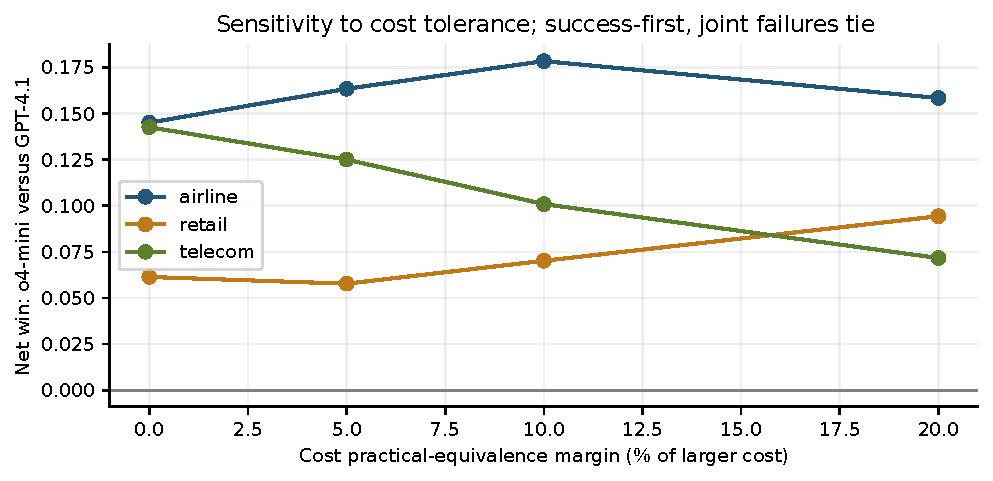
\includegraphics[width=\linewidth]{../plots/public_tolerance_sensitivity.pdf}
\caption{Cost-tolerance sensitivity under a fixed hierarchy. Changing
the threshold changes the preference estimand. All settings are reported;
none is selected because it favors a system.}
\end{figure}

The maintained CSV files include every primary contrast, cost tolerances
0, 0.10, and 0.20, reversed resource priority, common-seed pairing, and
all-pairs sensitivity. The internally dated analysis plan and amendment
are included. They are not a public preregistration. Some additional
exploratory suggestions in the feasibility audit remain unexecuted;
no conclusion relies on those suggested analyses.
